\newpage
\solutions{Gry}

%Source: https://om.mimuw.edu.pl/static/app_main/problems/om67_1.pdf Poland 2016 P1
\begin{problem}{1}
	Na tablicy napisano liczbę całkowitą dodatnią. W każdym ruchu zmazujemy napisaną liczbę $n$ na tablicy i piszemy nową liczbę. Jeśli $n$ była parzysta to piszemy na tablicy liczbę $\frac{1}{2}n$. Jeśli zaś liczba $n$ była nieparzysta, to zapisujemy jedną z liczb $3n - 1$ lub $3n + 1$. Czy -- niezależnie od tego, jaką liczbę zapisano na początku -- możemy, po skończenie wielu krokach, uzyskać na tablicy jedynkę?
\end{problem}

\answer{Jest to możliwe.}

\noindent
Wykażemy, że jeśli na tablicy znajduje się liczba $n \geqslant 2$, to zawsze jesteśmy w stanie sprawić, aby pojawiła się na tablicy dodatnia liczba całkowitej mniejsza od $n$. Rozpatrzmy dwa przypadki
\begin{itemize}
	\item Jeśli $n$ jest liczbą parzystą, to wystarczy zapisać liczbę $\frac{1}{2}n < n$.
	\item Gdy $n$ jest nieparzysta, to obie z liczb $3n + 1$ i $3n - 1$ są parzyste. Skoro różnią się o 2, to jedna z nich będzie liczbą podzielną przez $4$. Zapisujemy ją na tablicy, a następnie w dwóch kolejnych ruchach zapisujemy liczbę dwa razy mniejszą. Otrzymana liczba wyniesie co najwyżej
	\[
		\frac{3n + 1}{4} < \frac{4n}{4} = n.
	\]
\end{itemize}
Jako, że nie można ciągle zapisywać liczby mniejszej, gdyż zapisać można tylko liczby dodatnie całkowite, toteż kiedyś musimy zapisać liczbę $1$.

%Source: Lithuania 2010
% http://refkol.ro/matek/mathbooks/Grupe%20de%20performanta/Chapter5%20Games%20Aug%202014.pdf EX 9
\begin{problem}{2}
	W lewym dolnym rogu planszy $m \times n$ stoi pionek. W każdym ruchu może zostać on przesunięty o dowolną liczbę pól w górę lub o dowolną liczbę pól w prawo. Wygrywa gracz, który postawi figurę w prawym górnym rogu. Rozstrzygnąć dla jakich wartości $(m, n)$ pierwszy gracz ma strategię wygrywającą.
\end{problem}

\answer{Pierwszy gracz ma strategię wygrywającą wtedy i tylko wtedy, gdy $m \neq n$.}

\noindent
Analiza przykładowej planszy $7 \times 5$ została zobrazowana na poniższej tabelce. Litera $P$ oznacza, że jeśli pionek znajduje się na danym polu, to jest to stan przegrywający. Analogicznie $W$ oznacza stan wygrywający. Pole w prawym górnym rogu jest oczywiście stanem przegrywającym, gdyż jeśli przed ruchem tam znajduje się pionek, to gracz, którego jest kolej przegrał. Rozumując analogicznie jak w Przykładzie 2 otrzymamy poniższą tabelkę.
\begin{center}
\begin{tabular}{ |c|c|c|c|c|c|c|} 
 \hline
 W & W & W & W & W & W & P \\ 
 \hline
 W & W & W & W & W & P & W \\ 
 \hline
 W & W & W & W & P & W & W \\ 
 \hline
 W & W & W & P & W & W & W \\ 
 \hline
 W & W & P & W & W & W & W \\ 
 \hline
\end{tabular}
\end{center}

\noindent
Przejdźmy do rozwiązania zadania. Przyjmijmy, że pole w prawym górnym rogu ma współrzędne $(1, 1)$. Wówczas twierdzimy, że pole postaci $(a, b)$ jest przegrywające wtedy i tylko wtedy, gdy $a = b$. Wykażemy to indukcyjnie. Pole $(1, 1)$ jest przegrywające z definicji gry. Będziemy indukować się po sumie współrzędnych.

\vspace{10px}
\noindent
Jeśli gracz znajduje się na polu $(a, b)$, przy czym $a \neq b$, to może on przesunąć pionek na pole $(min(a, b), min(a, b))$, które jest stanem przegrywającym na mocy założenia indukcyjnego. Jeśli zaś gracz stoi na polu $(a, a)$, to jakiekolwiek pole, na które zostanie przesunięty pionek, nie będzie miało równych współrzędnych. Będzie więc stanem wygrywającym. Skoro więc każdy ruch doprowadza do stanu wygrywającego, to stan $(a, a)$ jest przegrywający.

\vspace{10px}
\noindent
Pozostaje tylko zauważyć, że dla $m \neq n$ wyjściowy stan jest wygrywający, a dla $m = n$ jest przegrywający. Toteż pierwszy gracz ma strategię wygrywającą jedynie dla $m \neq n$.

%Source: St. Petersburg 2001
% http://refkol.ro/matek/mathbooks/Grupe%20de%20performanta/Chapter5%20Games%20Aug%202014.pdf EX 10
\begin{problem}{3}
	Na tablicy zapisano liczbę $10000000$. W każdym ruchu, o ile przed nim była zapisana liczba $n$, gracz zastępuje ją liczbą $n - 1$ lub $\left\lfloor\frac{n + 1}{2}\right\rfloor$. Gracz, który zapisze liczbę $1$ wygrywa. Który z graczy – pierwszy czy drugi – ma strategię wygrywającą?
\end{problem}

\noindent
Wykażemy, że liczby parzyste są stanami wygrywającymi. Zauważmy, że liczba $2$ jest stanem wygrywającym, bo można ją zastąpić liczbą $2 - 1 = 1$. Załóżmy, że wszystkie liczby parzyste mniejsze niż $2a$ są stanami wygrywającymi.

\vspace{10px}
\noindent
Wykażemy, że liczba $2a + 2$ zapisana na tablicy również jest stanem wygrywającym. Rozpatrzmy dwa przypadki
\begin{itemize}
	\item Jeśli liczba $a + 1$ jest przegrywająca, to gracz wykonujący ruch może zastąpić liczbę $2a + 2$ przez liczbę $\left\lfloor\frac{2a + 3}{2}\right\rfloor = a + 1$ i w ten sposób umieścić przeciwnika w stanie przegrywającym.
	\item Załóżmy teraz, że liczba $a + 1$ jest wygrywająca. Wówczas gracz zastępuje liczbę $2a + 2$ liczbą $2a + 1$. Drugi gracz może zapisać albo liczbę $2a$ albo liczbę $a + 1$. Pierwsza z nich jest wygrywająca na mocy założenia indukcyjnego, a druga na mocy założenia z rozpatrywanego przypadku. W obu przypadkach gracz wykonujący ruch przy liczbie $2a + 2$ znów znajdzie się w stanie wygrywającym.
\end{itemize}

\vspace{10px}
\noindent
Wykazaliśmy, że liczby parzyste odpowiadają stanowi wygrywającemu, toteż skoro liczba $10000000$ jest parzysta, to pierwszy gracz ma strategię wygrywającą.

\begin{remark}
	Zauważmy, że nie wykazaliśmy nic o stanach, gdy na tablicy jest liczba nieparzysta. Nie było to jednak konieczne do rozwiązania powyższego zadania.
\end{remark}

\newpage

%Source: http://www.deltami.edu.pl/temat/matematyka/gry_zagadki_paradoksy/2017/12/31/Gry/ P4
\begin{problem}{4}
	Dwaj gracze na przemian stawiają kółko i krzyżyk w polach nieskończonej planszy. Gracz wygrywa, gdy istnieje kwadrat $2\times2$ ułożony z jego symboli. Wykazać, że drugi gracz może grać tak, aby pierwszy gracz nie był w stanie wygrać.
\end{problem}

\noindent
Podzielmy planszę na prostokąty $1 \times 2$ ułożone jak na rysunku -- boki wszystkich prostokątów o długości dwa są do siebie równoległe, ale żadne dwa z nich, które sąsiadują dłuższym bokiem, nie mają wspólnego wierzchołka.

\begin{center}
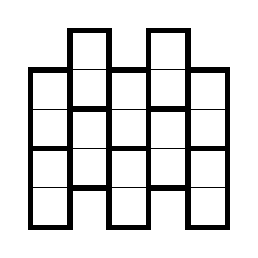
\begin{tikzpicture}[scale=0.5]

	\draw[line width=0.7mm] (0,0) -- (1,0) -- (1,2) -- (0,2) -- cycle;
	\draw (0,1) -- (1,1);
	\draw[line width=0.7mm] (0,2) -- (1,2) -- (1,4) -- (0,4) -- cycle;
	\draw (0,3) -- (1,3);

	\draw[line width=0.7mm] (1,3) -- (2,3) -- (2,5) -- (1,5) -- cycle;
	\draw (1,2) -- (2,2);
	\draw[line width=0.7mm] (1,1) -- (2,1) -- (2,3) -- (1,3) -- cycle;
	\draw (1,4) -- (2,4);

	\draw[line width=0.7mm] (2,0) -- (3,0) -- (3,2) -- (2,2) -- cycle;
	\draw (2,1) -- (3,1);
	\draw[line width=0.7mm] (2,2) -- (3,2) -- (3,4) -- (2,4) -- cycle;
	\draw (2,3) -- (3,3);

	\draw[line width=0.7mm] (3,3) -- (4,3) -- (4,5) -- (3,5) -- cycle;
	\draw (3,2) -- (4,2);
	\draw[line width=0.7mm] (3,1) -- (4,1) -- (4,3) -- (3,3) -- cycle;
	\draw (3,4) -- (4,4);

	\draw[line width=0.7mm] (4,0) -- (5,0) -- (5,2) -- (4,2) -- cycle;
	\draw (4,1) -- (5,1);
	\draw[line width=0.7mm] (4,2) -- (5,2) -- (5,4) -- (4,4) -- cycle;
	\draw (4,3) -- (5,3);
\end{tikzpicture}
\end{center}
Strategia drugiego gracza będzie następująca. Jeśli pierwszy gracz postawi swój symbol w jednym polu prostokąta, drugi gracz stawia swój symbol w drugim polu tego prostokąta. Kwadrat $2 \times 2$ zawiera pewien rozpatrywany prostokąt w całości. Jednak sytuacja, w której jeden prostokąt zawiera dwa jednakowe symbole się nie zdarzy. Stąd rozpatrywana strategia spełnia warunki zadania.


%Source: Russia 2021 10.5
% https://artofproblemsolving.com/community/c6h2534986p21567788
\begin{problem}{5}
	Nauczyciel wraz z 30 uczniami gra w grę na nieskończonej kartce w kratkę. Zaczyna on, po czym ruch wykonuje każdy z 30 uczniów, po czym znów nauczyciel, po czym uczniowie i tak dalej. W każdym ruchu należy pokolorować jeden z boków kratki, który nie został wcześniej pokolorowany. Nauczyciel wygrywa, gdy na planszy znajduje się prostokąt $2 \times 1$ lub $1 \times 2$, że wszystkie jego boki są pokolorowane, ale odcinek wewnątrz niego nie jest.
\end{problem}

\noindent
Strategia nauczyciela jest następująca. Rysuje on obwód kwadratu $n \times n$ w pierwszych $4n$ ruchach, w międzyczasie uczniowie zamalują $4n \cdot 30$ odcinków. Wówczas wewnątrz kwadratu znajduje się $2n(n - 1)$ odcinków. Jeśli $2n(n - 1) > 4n \cdot 30$, do czego wystarczy wziąć odpowiednio duże $n$, to liczba odcinków wewnątrz kwadratu będzie większa niż liczba odcinków pomalowana przez uczniów. Toteż będzie co najmniej jeden odcinek wewnątrz tego kwadratu, który nie jest pomalowany.

\begin{center}
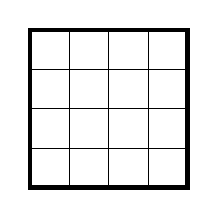
\begin{tikzpicture}[scale=0.5]
	\draw[line width = 0.6mm] (0,0)--(4,0)--(4,4)--(0,4)--cycle;
	\draw (0,1)--(4,1);
	\draw (0,2)--(4,2);
	\draw (0,3)--(4,3);
	\draw (1,0)--(1,4);
	\draw (2,0)--(2,4);
	\draw (3,0)--(3,4);
\end{tikzpicture}
\hspace{40px}
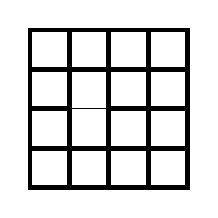
\begin{tikzpicture}[scale=0.5]
	\draw[line width = 0.6mm] (0,0)--(4,0)--(4,4)--(0,4)--cycle;
	\draw[line width = 0.6mm] (0,1)--(4,1);
	\draw[line width = 0.6mm] (0,2)--(1,2);
	\draw (0,2)--(4,2);
	\draw[line width = 0.6mm] (2,2)--(4,2);
	\draw[line width = 0.6mm] (0,3)--(4,3);
	\draw[line width = 0.6mm] (1,0)--(1,4);
	\draw[line width = 0.6mm] (2,0)--(2,4);
	\draw[line width = 0.6mm] (3,0)--(3,4);
\end{tikzpicture}
\end{center}

\vspace{10px}
\noindent
Następnie nauczyciel w każdym ze swoich ruchów maluje pewien odcinek wewnątrz narysowanego kwadratu. Jako że liczba odcinków wewnątrz rozpatrywanego kwadratu jest skończona, to w końcu zarówno obwód, jak i wszystkie odcinki wewnątrz niego będą pokolorowane. Więc w pewnym momencie dokładnie jeden z odcinków wewnętrznych nie był pokolorowany -- wówczas musiał istnieć szukany prostokąt bez środkowego odcinka.

%Source:
% https://www.math.hkust.edu.hk/excalibur/v7_n5.pdf EX 4
\begin{problem}{6}
	$20$ dziewczyn usiadło w kółku. Na początku jedna z nich trzyma $N < 19$ kamieni. W każdym ruchu jedna z dziewczyn, która posiada co najmniej dwa kamienie daje po jednym każdej ze swoich sąsiadek. Gra kończy się, gdy każda z dziewczyn trzyma co najwyżej jeden kamień. Wykazać, że gra musi się skończyć po skończonej liczbie ruchów.
\end{problem}

\noindent
Załóżmy nie wprost, że gra może trwać w nieskończoność.
Ponumerujmy dziewczyny liczbami od $1$ do $20$.
Przyjmijmy, że na każdym kamieniu są miejsca na zapisanie dwóch liczb. Jeśli pewna dziewczyna $a$ przekaże dziewczynie $b$ kamień po raz pierwszy, to o ile na kamieniu nie jest nic zapisane, to zapisuje się tam numery $a$ i $b$. 
Jeśli pewna dziewczyna musi przekazać kamień swojej sąsiadce, to jeśli dysponuje kamieniem z zapisanymi numerami swoimi i sąsiadki, to przekaże jej właśnie go.

\vspace{10px}
\noindent
Należy zauważyć, że jeśli kamień jest podpisany numerami $a$ oraz $b$, to od momentu podpisania będzie posiadała go albo dziewczyna o numerze $a$, albo dziewczyna o numerze~$b$. W momencie podpisania tak istotnie jest. Jeśli jedna z tych dziewczyn ma przekazać kamienie sąsiadkom, to rozpatrywany kamień będzie przekazany do drugiej dziewczyny ze zbioru $\{a, b\}$.

\vspace{10px}
\noindent
Skoro jest $N < 19$ kamieni oraz $20$ kolejnych par dziewczyn, to będzie istnieć para kolejnych dziewczyn, która nie będzie miała kamienia podpisanego swoimi numerami. Załóżmy, że jedna z tych dziewczyn ma numer $a$. Wówczas ani razu nie przekaże ona swoich kamieni nikomu, bo w przeciwnym wypadku przekazałaby go drugiej z rozpatrywanych dziewczyn.


\vspace{10px}
\noindent
Załóżmy, że dziewczyna o numerze $k$ przekazała kamienie sąsiadkom skończenie wiele razy. Wówczas jeśli dziewczyna o numerze $k - 1$ (oczywiście rozpatrzamy numery modulo~$20$) robiłaby to bez końca, to w pewnym momencie dziewczyna o numerze $k$ miałaby więcej niż $19$ kamieni. Stąd jeśli $k$ wykonała skończenie wiele ruchów, to $k - 1$ też. Wiemy, że dziewczyna o numerze $a$ wykonała zero, czyli skończenie wiele ruchów. Rozumując indukcyjnie dowodzimy, że każda dziewczyn mogła wykonać skończenie wiele ruchów, co kończy dowód.